% AER-Article.tex for AEA last revised 22 June 2011
\documentclass[AER]{AEA}

\usepackage{tikz,tikz-qtree}
\usepackage{graphicx}
\usepackage{float}
\usepackage{hyperref}
\usepackage{multirow}
\usepackage{makecell}
\usepackage{lipsum} 
\usepackage{threeparttablex,booktabs}
\usepackage{cleveref}
\usepackage{subcaption}
\usepackage{minted}
\usepackage[parfill]{parskip} % no indent and line break for each paragraph 
\usepackage[hang]{footmisc} % no indent for footnote
\setlength\footnotemargin{1em}  % default value: 1.8em

%\renewcommand{\thefootnote}{\roman{footnote}}

% The mathtime package uses a Times font instead of Computer Modern.
% Uncomment the line below if you wish to use the mathtime package:
%\usepackage[cmbold]{mathtime}

% Note: you may use either harvard or natbib (but not both) to provide a wider
% variety of citation commands than latex supports natively. See below.

% Uncomment the next line to use the natbib package with bibtex
%\usepackage[round]{natbib}
% \bibliographystyle{plainnat}

\usepackage[round]{natbib} 
\setcitestyle{aysep={,}} 
\bibliographystyle{dcu}

% Uncomment the next line to use the harvard package with bibtex
%\usepackage[abbr]{harvard}

% This command determines the leading (vertical space between lines) in draft mode
% with 1.5 corresponding to "double" spacing.
\draftSpacing{1.5}

% use package subcaption modifies the AEA style caption; reset the style here
\captionsetup[table]{labelfont={sc,small}, textfont={sc,small}, labelformat=simple, labelsep=period}
\captionsetup[figure]{labelfont={sc,small}, textfont={sc,small}, labelformat=simple, labelsep=period}
\captionsetup[subfigure]{labelfont=normalfont, textfont=normalfont}

% define OliveGreen color
%\definecolor{OliveGreen}{rgb}{0,0.6,0}


\begin{document}

\title{MODELLING THE POTENTIAL IMPACTS OF FINANCIAL LIBERALIZATION IN CHINA}
\shortTitle{Financial Liberalization in China}
\author{Zeming Wang,\ \textit{Supervised by} Paul Gretton}
\date{\today}
\pubMonth{OCT.}
\pubYear{2017}
%\Keywords{}

\begin{abstract}
\noindent
China has experienced exceptional economic growth in the past three decades 
driven by policy reforms and economic liberalization. 
However, reforms in financial sectors have been lagging behind real sectors 
and there are still extensive regulations repressing the financial system.
This paper reviews the theories of financial development and economic growth, 
and examines the facts and consequences of financial repressive policies 
undertaken in China. 
Then several simulations are performed to project the potential impacts of 
financial market liberalization reforms. 
The simulations found China could remarkably increase its national output 
and capital accumulation due to such reforms, and most regions in the 
world would benefit as well. 
However, financial liberalization should be undertaken prudently together 
with risk management to mitigate possibly disruptive short-run fluctuations 
in the Chinese economy.
\end{abstract}


\maketitle

\section{Introduction}

China has experienced exceptional economic growth in the past three decades 
driven by massive policy reforms and economic liberalization.
However, liberalization in China's financial sectors has lagged 
the pace of change compared to real sectors such as manufacturing, 
construction, and technology. 
Despite rapidly growing demands for financial 
services, the financial system remains highly restricted. 
Restrictive financial policies are usually justified to maintain  
stability of the economy. 
However, such policies inhibit the proper functioning of the markets,  
which inevitably causes inefficiency and resource mismatches. 
To show the importance and urgency of financial reforms, it is necessary 
to review the theories of financial development and economic growth, 
and examine China's prevailing economic conditions. 

Economists' have different views on the importance of financial 
systems to economic growth. Classical school economists, though agree on the 
functions of the financial system to facilitate transactions, generally 
do not adopt the idea that the financial system plays a key role to economic success, 
since economic growth  essentially takes place in real sectors 
(for example, money is neutral). 
But, modern economists have increasingly unraveled the importance of the 
financial system for economic growth \citep{boyd1986,levine1991,bekaert2001}.
To briefly summarize, financial markets and intermediaries have been identified 
as functioning to mobilize savings, allocate resources, and 
reduce transaction and information costs, while facilitating liquidity, 
ameliorating risk, and exerting corporate controls. 
While a well-functioning financial system could allocate resources 
efficiently and promotes capital accumulation and potentially technological  
innovation, a mal-functioning financial system undermines these channels 
and hinders economic growth. 

However, most developing countries tends to place  
restrictions on their financial systems, such as imposing  
tariffs to protect infant industries, and artificially lowering  
interest rates to provide cheap capital to nascent enterprises. 
China is a good example of such restrictive policies:  
state-owned banking system used to channel the government's industrial  
policies, highly regulated capital accounts to mitigate  
fluctuations of the exchange rates caused by cross-border capital 
flows, and various industry entry barriers to unduly reduce competition.
These policies could be helpful with maintaining the stability of the economy 
in countries with fragile financial systems. 
But as many researchers have pointed out,  as developing economies mature,
these repressive policies can be more prohibitive than productive.
For example, state-owned banks and controlled interest rates have caused 
significant mismatches in resource allocation and imbalances in development 
among economic sectors. 
Industry entrance barriers stifle competition in some industries,  
resulting in inefficiency and inequality. 
Thus, the consensus in China is to further liberalize the financial system 
and with this improve efficiency of the economy.

To estimate the potential impacts of financial liberalization on China, 
several simulations are carried out using the GTAP general equilibrium 
model of the global economy. 
In the model, policy reforms are modelled as ``shocks". 
We simulate three scenarios in this paper: 
a reduction in required rate of return on capital, 
an increase in productivity of financial services, 
and an increase in productivity of capital. 
This scenario conjectures that productivity improvements in the use of 
capital are possible for those sectors dominated by state-owned enterprises.
The simulations project a remarkable increase in China's real GDP -- 
almost 5\% and an even larger increase in the total capital 
accumulation -- nearly 12\%. 
Other countries, such as Australia and the United States,  are projected to 
benefit from China's reform as well.
% The simulations also suggest productivity improvements for those 
% sectors dominated by state-owned enterprises. 

China is now in a critical transition from a middle-income to 
a higher-income economy. To sustain growth and improve efficiency, it is 
essential for the government to further financial reform and liberalization.
But to push forward such reform also poses challenges to Chinese policy makers 
-- to push forward financial liberalization while managing to control 
the potential risk that might be induced by such policies.   
Therefore, it is suggested in this paper that financial liberalization be undertaken 
together with proper risk management.
The remainder of this paper is organized o address these issues in more depth.
\Cref{sec:theory} reviews the theories of financial development and 
economic growth.
\Cref{sec:facts} examines the financial repression situations in 
China and points out the necessity of financial liberalization. 
\Cref{sec:model} uses GTAP model to simulate the potential impact of 
financial liberalization in China. 
\Cref{sec:policy} addresses some policy concerns, alerts the potential 
risks and concludes the essay.\\


% But as the economy is transitioning from its past quantity growth mode 
% to a quality growth mode, financial restrictive policies appear to be 
% more hindering than ever to achieve efficient allocation of resources 
% in the economy. 


% China has been no tenderfoot in handling large global trade transactions for
% many years, with its largest export and second largest import volume in the
% world to-day. Meanwhile, China has been very scrupulous in regulating its
% capital account. The liberalization of China's capital account follows tardily
% to its current account openness, even though its capital account is already
% large by global standards, which roughly accounts for 6 per cent of global
% cross-border financial transactions (Finsia 2014).

% The growing need for cross-border capital move, as well as the domestic urge for
% accelerating the pace of financial system reform, calls for further
% liberalization of China's capital account.


\section{Finance and Economic Growth}
\label{sec:theory}

The relationship of financial development and economic growth has been
intensively studied by economists in the past few decades. Financial markets and
intermediaries have been identified helping to mobilize savings and allocate
resources to productive usage, improving access to capital and lowering
transaction and information cost, facilitating market liquidity and risk
management, which all promotes capital accumulation and speed up productivity
improvements. Though there are economists against the over-stress of the role of
finance in economic development \citep{lucas1998} and some address the
instability and fragility of immature financial systems \citep{stiglitz2000},
the basic arguments for financial development and economic growth widely accepted. 

The function of financial intermediaries to reduce transaction costs was
uncovered back in Adam Smith's time. Smith conceived the idea that money was
preferred over barter because the use of money would reduce transaction costs,
while a reduction of transaction costs would encourage a greater scale of
specialization because specialization requires more transactions than
autarkic-style production, and finally productivity would be promoted with more
specialized labor.
% \begin{quote}
% ``In order to avoid the inconvenience of such situations, every prudent man in
% every period of society, after the first establishment of the division of
% labour, must naturally have endeavoured to manage his affairs in such a manner,
% as to have at all times by him, besides the peculiar produce of his own
% industry, a certain quantity of some one commodity or other, such as he imagined
% few people would be likely to refuse in exchange for the produce of their
% industry.'' \citep{smith1776}
% \end{quote}

Widespread financial institutions, including but not limited to monetary institutions, all help to reduce transaction costs some ways or other. 
For example, banking systems reduce the transaction costs of cross-region payments. 
Without proper financial intermediation, cross-industry or cross-region transactions 
would be prohibitively costly, which would impede greater specialization and stifle
productivity growth. 

Joseph Schumpeter expounded the role of financial intermediaries to economic
development in his book \textit{The theory of economic development}
\citep{schumpeter1934}. 
Schumpeter viewed economic development, in a capitalism economy, as the
process of continuously adopting newly created kinds of goods and new combinations
of means of production. Innovative entrepreneurs play a central role in this
process, and so do bankers and other financiers. Bankers facilitate
entrepreneurs' innovation activity by issuing credit to them. In this process,
bankers are not simply playing an intermediation role, but they are as creative as
entrepreneurs, for they bid for higher returns on capital and strive to find out
the most productive businesses. Bankers are themselves a kind of
innovative entrepreneurs, for they innovate to channel the resources of a
society to the most productive use. %
% \begin{quote}
% ``Financial institutions and practices enter our circle of problems in three
% ways: they are `auxiliary and conditioning'; banking may be the object of
% entrepreneurial activity, that is to say, the introduction of new banking
% practices may constitute enterprise; and bankers (or other `financiers') may use
% the means at their command in order to embark upon commercial and industrial
% enterprise themselves." \citep{schumpeter1947}
% \end{quote}
Thus, the development of financial systems facilitates efficient investment and
promotes technological innovation. The function is not limited to banks, other
financial intermediaries as well as financial markets also support economic
development in either direct or indirect ways.
% \begin{quote}
% ``Stock exchange speculation, especially, and the speculative holding of newly
% issued stock were in all countries largely financed by banks, which, therefore,
% always served the purpose of financing long-time investment, at least in this
% indirect way, even if in no other." \citep{schumpeter1939}
% \end{quote}

Modern researchers have developed more comprehensive theories on how financial
system facilitates economic growth. \cite{boyd1986} addressed that the cost of
information acquisition necessitates the emergence of financial intermediaries.
The reasoning is, without proper financial intermediaries, everyone has to pay
the cost of acquiring information about investment opportunities.  
The emergence of financial intermediaries economize the information acquisition
process and improve the efficiency of resource allocation. This view
augments Schumpeter's financial innovation argument with both putting 
an emphasis on the information discovery role of financial system, that is
discovering the most promising firms and managers and channeling capital to the
most productive use. 

Multiple researchers, \cite{diamond1983}, \cite{levine1991},
\cite{bencivenga1991} addressed the liquidity facilitating role of financial
institutions in promoting economic growth. The connection between liquidity and
economic growth is due to the tension between the long-run commitment of capital
required by some investment and the reluctance of savers to
relinquish their capital for a long time. For instance, if each saver were to
invest on their own, they would have to make long-run investment very cautiously
and have to at least reserve a proportion of their savings in liquid form. With
well-functioned financial markets and intermediaries facilitating liquidity,
more capital can be directed to long-run investment than it would have been
otherwise. For example, in liquid stock markets where shareholders can readily
sell their shares, investors would be more likely to invest in firms' equity for
not being worried about reclaiming their purchasing power when they need it.
Banks that offer demand deposits to their savers could hold mixed-term
portfolios which meet the savers' demand for liquidity on the one hand, and
optimally invest in long-run projects on the other. 
In this way, financial institutions that facilitate liquidity promote long-run 
investment in an economy and therefore contribute to long-run economic growth. 

Financial systems are also well-known for their function of mobilizing savings,
that is pooling capital from disparate savers for investment. By effectively
pooling capital, financial systems not only facilitate large investment and
capital accumulation, but also promote the use of costly technologies which  
could potentially raise economic growth \citep{mckinnon1973}. 
% The role of financial systems in promoting better technology use is 
% illustrated by \cite{mckinnon1973}:
% \begin{quote}
% ``The important point, however, is the virtual impossibility of a poor farmer's
% financing from his current savings the whole of the balanced investment needed
% to adopt the new technology. Access to external financial resources is likely to
% be necessary over the one or two years when the change takes place. Without this
% access, the constraint of self-finance sharply biases investment strategy toward
% marginal variations within the traditional technology."
% \end{quote}

% \cite{hicks1969} even argued without a finance system that efficiently
% mobilizing savings, the industrial revolution would had happened in Britain in
% eighteenth century. His essential argument is that the products manufactured in
% the early phase of industrial revolution had been invented much earlier.
% However, the manufacturing of these products required large-scale and long-run
% commitment of capital. Without a highly sophisticated financial system to
% mobilize savings and facilitate investment, it would be impossible for
% technology innovation itself to spark the industrial revolution.

% Financial markets have also been identified having the capability of monitoring 
% managers and exerting corporate controls over companies \citep{jensen1976}.
% For example, shareholders can takeover under-perform companies through 
% buying their shares in stock markets and replace unqualified managers. 
% The threat of being took-over exerts an invisible monitoring over managers 
% of public firms, which helps align managers' incentives with shareholders' 
% interests. 

While free trade in goods across border is well known to promote global labour 
specialization and raise economic development, free flow of capital optimizes 
capital allocation in a global scale. As \cite{bekaert2001} and \cite{henry2000} 
showed in their research, capital account liberalization has a significant 
impact on the reduction of the cost of capital, closing the wedge between 
external and internal capital, and thereby inducing more investment. 
A freely opened capital account has also been identified to promote 
domestic financial development \citep{love2003}, for it promotes competition 
among financial institutions. 
An opened capital account also imposes ``discipline" and forces good economic 
policies domestically, to avoid capital flight and attract foreign investment.
However, it must also be noted that, free flow of capital is not without 
defects. As \cite{stiglitz2000} pointed out, freely opened capital account 
``exposes countries to vicissitudes associated with changes in economic 
circumstances outside the country''. It could be detrimental especially to 
countries with a fragile financial system, because pro-cyclical capital 
flows would exacerbate economic fluctuations. 

Despite the multiple benefits of an efficient financial system to economic growth, 
restrictions on financial system functioning are commonplace in developing 
economics including through interest rate controls, capital flow controls,  
and government designating investments.
While the merits of these restrictions are questionable, 
the hindrance they place on the well-functioning of capital markets is certain. 
As \cite{mckinnon1973} pointed out, the fragmentation in the capital market 
as the result of repressive financial policies ``causes the misuse of 
labor and land, suppresses entrepreneurial development, and condemns 
important sectors of the economy to inferior technologies''. 
The specific example of China in this concern is discussed in detail 
in the following section.\\

% While free trade of goods across borders is known to promote labour specialization 
% and improve productivity worldwide, free flow of capital helps to allocate 
% capital efficiently on a global scale. 

\section{Financial Repression in China}
\label{sec:facts}

\subsection{Overall financial development}

It is not easy to measure the overall financial development of a country,
given the complexity of financial system. Traditional measures make
use of ratios like total credit to GDP, or stock market capitalization to GDP.
However, these measures only address certain aspects of a financial system, and
inevitably overlook other dimensions. To help fill this gap, an IMF working paper,
constructed a comprehensive index for financial system development
worldwide, which sheds light on the relative financial development of China
compared to other countries in the world \citep{sviry2016} . 

The index is constructed using 33 years of annual data between 1980 and 2013 for
183 countries worldwide by measuring three dimensions -- depth, access and 
efficiency -- of both financial institutions and financial markets. 

% The construction of the financial development index is illustrated in 
% \autoref{fig:pyramid}.

% The depth of financial institutions is measured by credit to GDP ratio, 
% pension fund assets to GDP ratio, and alike; the accessibility is measured by
% the density of bank branches or ATMs; and the efficiency is measured by 
% net interest margin, lending-deposits spread, etc. For financial markets,
% the depth is measured by stock market capitalization to GDP ratio, total 
% debt securities to GDP ratio, etc.; the accessibility is measured by, 
% for example, the total number of issuers of debt; and the efficiency is measured 
% by indicators like stock market turnover ratio. 

% \begin{quote}
% ``Financial development is defined as a combination of depth (size and
% liquidity of markets), access (ability of individuals and companies to access
% financial services), and efficiency (ability of institutions to provide
% financial services at low cost and with sustainable revenues, and the level of
% activity of capital markets)." \citep{sviry2016}
% \end{quote}
%
% While depth of financial institutions is measured by ratios including
% private-sector credit to GDP, pension fund assets to GDP, mutual fund assets to
% GDP and insurance premiums to GDP; accessibility measured by bank branches and
% ATMs per 100 thousand adults; efficiency measured by net interest margin,
% lending-deposits spread, non-interest income to total income, overhead costs to
% total assets, return on assets and return on equity.
%
% Depth of financial markets is measured by stock market capitalization to GDP,
% stocks traded to GDP, international debt securities of government to GDP, total
% debt securities of financial corporations to GDP, total debt securities of
% nonfinancial corporations to GDP; accessibility measured by\% of market
% capitalization outside of top 10 largest companies, and total number of issuers
% of debt; efficiency measured by stock market turnover ratio.

% \begin{figure}[!htb]
% \centering
% \begin{tikzpicture}[level distance=40pt]
% %   \tikzset{edge from parent/.style={draw,->, edge from parent path={
% %            (\tikzparentnode.south) -- +(0,-8pt) -| (\tikzchildnode)}}}
% %   \tikzset{every tree node/.style={align=center}}
% %   \tikzset{every level 1 node/.style={font=\small, text width=4cm}}
% %   \tikzset{every level 2 node/.style={font=\small, text width=4cm}}
%   \tikzset{every tree node/.style={font=\small}}
%   \Tree [.{Financial Development Index}
%             [.{Financial Institutions}
%                 [.{Depth} ]
%                 [.{Access} ]
%                 [.{Efficiency} ]
%             ]
%             [.{Financial Markets}
%                 [.{Depth} ]
%                 [.{Access} ]
%                 [.{Efficiency} ]
%             ]
%         ]
% \end{tikzpicture}
% \caption{Financial Development Index Pyramid}
% \begin{minipage}{0.8\textwidth}
% \begin{center}
% \notesize{\textit{Source}: \cite{sviry2016}, 
% IMF staff, based on Čihák and et al. (2012)}
% \end{center}
% \end{minipage}
% \label{fig:pyramid}
% \end{figure}

\autoref{fig:findev} shows the Financial Development Index together with 
two sub-indices -- Financial Institution Index and Financial Market Index 
for a selected list of countries. 
China scores 0.572 for overall financial development, 
which is approximately equivalent to only 65\% of the financial development 
level of Australia or the United States. China not only falls 
behind developed countries, but even behind other developing countries such as 
Malaysia and Thailand. 
\autoref{fig:findev} also shows that China's financial market development 
scores higher than its financial institutions, which is a reflection of China's 
sluggish financial institution reform relative to its financial market reform. 

\begin{figure}[!htb]
\centering
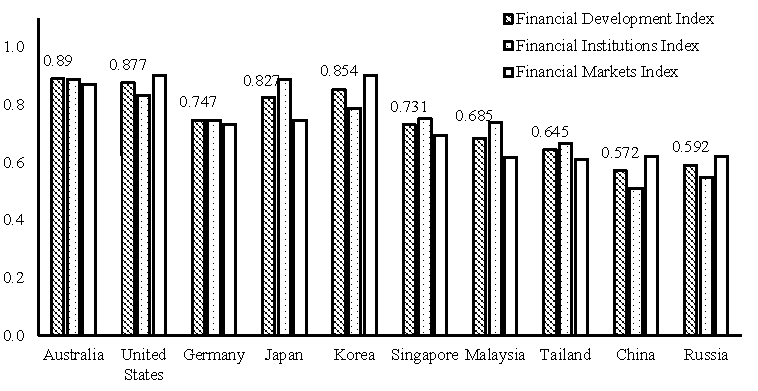
\includegraphics[scale=1]{fig/findev.pdf}
\caption{Financial Development Index for Selected Countries}
\begin{figurenotes}[Source]
Based on \textit{2013 Country Rankings on Financial Development} by
\cite{sviry2016}.
\end{figurenotes}
\label{fig:findev}
\end{figure}

% Another metric of financial development is through the overall cost of capital in 
% an economy. Although financial repression situations vary from country to country, 
% the overall effect of repression is to limit the financial resources available 
% to investors and raise the cost of capital. 
% Though there is no direct measure of the cost of capital, the 10-year treasury yield 
% can be used as a proxy if assuming investors could arbitrage between financial and 
% physical assets. 

% \begin{figure}[!htb]
% \centering
% \includegraphics[scale=1]{fig/treasury.pdf}
% \caption{10-Year Treasury Yield: China vs. the US}
% \label{fig:t-yield}
% \begin{figurenotes}[Source]
% National Inter-bank Funding Center (China), Federal Reserve Board (US).
% \end{figurenotes}
% \end{figure}

% \autoref{fig:t-yield} shows that there is a persistent wedge (1 percentage point on average) 
% of the treasury yield between the two countries since 2010 
% (during the GFC, China pegged its currency exchange rate to the U.S. dollar, 
% so the treasury yields of the two countries converged; the pegging exchange 
% rate was not freed until mid-2010).
% The persistent wedge reflects the risk premium of China against the US. 
% If China were to reform its financial repression situations, it would be expected 
% to reduce the wedge, lower the overall cost of capital and induce more investment. 

\begin{figure}[!htb]
\centering
\begin{subfigure}{.5\textwidth}
\centering
\includegraphics[scale=.5]{fig/invest.pdf}
\caption{Gross capital formation (\% of GDP)}
\label{fig:invest}
\end{subfigure}%
\begin{subfigure}{.5\textwidth}
\centering
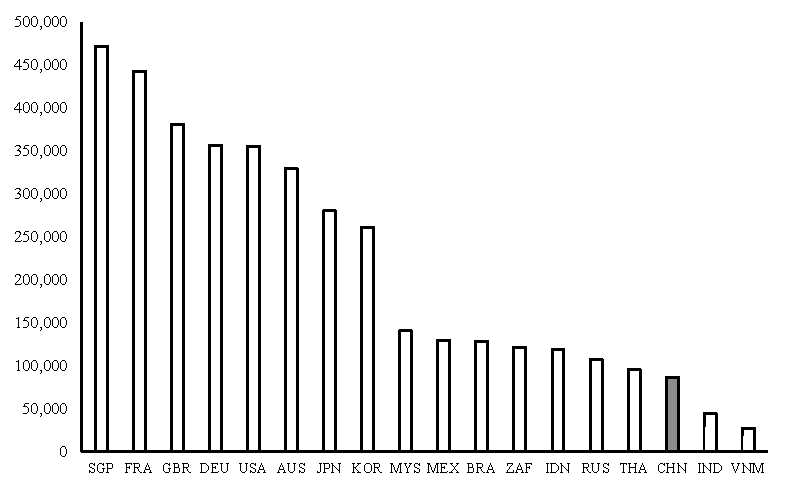
\includegraphics[scale=.5]{fig/capital-pc.pdf}
\caption{Capital stock per worker (2014)}
\label{fig:capital-pc}
\end{subfigure}
\caption{Investment and Capital per Worker}
\begin{figurenotes}
Capital values are converted using purchasing power parity, and shown in 2011 US\$. 
\end{figurenotes}
\begin{figurenotes}[Source]
The World Bank, Penn World Table Version 8.0.
\end{figurenotes}
\end{figure}

During the past decades, China has been heavily relying on government-led
investment and infrastructure building. 
% Although capital accumulation has increased dramatically in China 
% (\autoref{fig:invest}), the capital stock per worker is still well below 
% the level of developed countries (\autoref{fig:capital-pc}).
As shown in \autoref{fig:invest}, China has a higher investment to GDP ratio 
than other regions, but the ratio has been declining in recent years. 
The combined financial market restrictions and high investment has resulted in 
large amount of inefficient investment in government favoring sectors, 
while many private enterprises and especially small businesses have been 
suffering from insufficient funding. 
To further increase overall capital per worker in competitive actives 
and improve productive efficiency, 
China needs to transform its policy-oriented investment 
strategy to a profit-oriented one. 
This would require further financial reform 
and liberalization in the economy to achieve more efficient allocation of 
resources. \\

\subsection{Repressive financial institutions}

To drill down into the financial repression status in China, this section takes 
a close look at China's domestic banking system, because banks almost dominate 
the financial system in China.

The state-owned banks are arguably the most entrenched and criticized 
segment of China's banking system. The state controls almost 70\% of 
all the assets through state-owned commercial banks and policy banks 
(\autoref{tab:banks}).

%
% As shown in \autoref{tab:banks}, 
% commercial banks either directly owned by the state or 
% indirectly controlled by the state as the largest shareholder account for 
% 64\% of the total banking assets. Taking into account the policy banks 
% -- special purposed state-controlled banks -- the state controls 72\% of 
% all the assets. Foreign banks' share is only 1.68\%. 
% The data shown in \autoref{tab:banks} was collected in 2009. 
% Though China took the agenda to allow private banks in the past few years, 
% the licences are extremely limited and only granted to designated qualified 
% entrepreneurs. 
% Even nowadays, the share of private banks is still negligible, 
% while state-owned banks dominate the system. 

\begin{table}[!htb]
\begin{threeparttable}
\caption{China's Banking Institutions (2009)}
\label{tab:banks}
\def\theadset{\def\arraytretch{2}}
\def\arraystretch{1.2}
\small
\begin{tabular}{lcccc}
\hline\hline
& & & \multicolumn{2}{c}{\makecell{Asset\\(RMB trillion)}} \\\cline{4-5}
& Number & Share (\%) & Amount & Share (\%) 
\\
\hline
Policy banks & 3 & 0.05 & 6.95 & 8.63 
\\
State-owned commercial banks & 4 & 0.07 & 39.04 & 48.47 
\\
\makecell[l]{Joint-stock commercial banks,\\State as largest shareholder} 
 & 11 & 0.20 & 12.59 & 15.63 
\\
Others & 2 & 0.04 & 2.01 & 2.50 
\\
\hline
\multicolumn{5}{l}{Other banks}
\\
City commercial banks and credit unions & 158 & 2.80 & 5.71 & 7.09 
\\
Rural commercial banks and credit unions & 5241 & 93.02 & 8.64 & 10.73 
\\
Postal savings bank & 1 & 0.02 & 2.70 & 3.35 
\\
Foreign banks & 32 & 0.57 & 1.35 & 1.68 
\\
Non-bank institutions & 182 & 3.23 & 1.55 & 1.92 
\\
\hline
Total & 5634 & 100.00 & 80.53 & 100.00 
\\
\hline\hline
\end{tabular}
\begin{tablenotes}[para,flushleft]
\footnotesize
\emph{Source:} Data from \cite{deng2011}.
\end{tablenotes}
\end{threeparttable}
\end{table}

For decades, China's government has taken advantage of the state-owned banking 
segment to channel financial resources to its preferred sectors. With the 
central bank (PBoC) controlling interest rates (until 2015), 
the state-owned banks can acquire savings at an artificial low cost 
on the one hand, and lend the capital cheaply to government designated 
projects on the other. 
Instead of being a competitive industry seeking best return on investment, 
the banking system in China is more like a proxy for the government's 
industry policies. 
The major beneficiaries of such policies are the state-owned enterprises (SOE), 
which receive nearly 60\% of all the loans.
Loans to private enterprises only account for 30\%, and foreign enterprises 
for the remaining 10\%.

%\footnote{Data from CEIC and People's Bank of China.}

% \begin{figure}[!htb]
% \centering
% \includegraphics[scale=1]{fig/loans.pdf}
% \caption{China Bank Loans to Types of Enterprises}
% \begin{figurenotes}[Source]
% Based on data from CEIC, People's Bank of China.
% \end{figurenotes}
% \label{fig:loans}
% \end{figure}

% \autoref{fig:loans} shows the shares of banking loans to different types of 
% enterprises. The major beneficiaries are the 
% state-owned enterprises (SOEs), who receive nearly 60\% of all the loans, 
% while loans to private entrepreneurs only take about 20\%. 

The result is the excess investment in SOEs, often in low quality investments,
on the one hand, and the inadequate funding and higher cost of capital for private 
enterprises on the other. Private enterprises, especially small ones, 
that cannot obtain loans from formal commercial banks, go to local 
private lending companies, where a much higher interest rate is charged 
than available from formal banks. 
This results in a fragmentation of interest rates as 
shown in \autoref{fig:lrate}. While the official benchmark interest rate 
stays as low as 4\%, the private lending rate has never been 
below 15\%. The P2P network lending rate has declined significantly, 
but is still above 10\%. As a comparison, the P2P network lending rate 
of major platforms in the United States is only 6\%. 
In addition, the inflexible official rate often results in negative real 
interest rate (\autoref{fig:realr}), which impairs the interest of savers.

\begin{figure*}[!htb]
\centering
\begin{subfigure}{.5\textwidth}
\centering
\includegraphics[scale=.5]{fig/lrate.pdf}
\caption{Various interest rates}
\label{fig:lrate}
\end{subfigure}%
\begin{subfigure}{.5\textwidth}
\centering
\includegraphics[scale=.5]{fig/realr.pdf}
\caption{Real interest rate}
\label{fig:realr}
\end{subfigure}
\caption{Fragmentation of Interest Rates}
\begin{figurenotes}
Wenzhou private lending rate is based on the Wenzhou composite lending rate index,
which is the private lending rate in Wenzhou and is published officially by the 
government of Wenzhou. P2P network lending rate is the average lending rate of 
online P2P platforms. China's central bank directly controls commercial banks' 
lending rate, which is shown as the benchmark rate.
\end{figurenotes}
\begin{figurenotes}[Source]
CEIC, People's Bank of China, The World Bank.
\end{figurenotes}
\end{figure*}

The fragmentation of interest rates, and especially the high lending 
interest rate for small enterprises, is hindering the development of small 
businesses, while the artificially lowered formal rate channels more 
resources to SOEs and results in excess capital investment and low 
efficiency in industries dominated by SOEs. \autoref{fig:roa} 
calculates the average return on asset (ROA) of 10 major sectors 
listed on China's stock market and shows the imbalance of returns 
among them. Sectors that are dominated by SOEs such as energy, 
materials, industries, telecom, financials, and utilities 
generally average to much lower returns; and the returns have 
experienced sharp decline over the last decade. While the sectors 
mainly dominated by private enterprises such as consumer goods 
and technology providing much higher and relatively stable returns  
over time are in evidence.
 
\begin{figure}[!htb]
\centering
\includegraphics[scale=1]{fig/roa.pdf}
\caption{Return on Asset by Sectors}
\begin{figurenotes}
The values reported here are calculated from the data of the companies listed 
on the stock market. The number of companies consisted in each sector are 
also meaningful, and are thus reported here: energy (84), materials (537), 
industries (810), consumer discretionary (534), consumer staples (211), 
health care (226), finance and real estate (224), technology (464), 
telecom (94), and utilities (96).
\end{figurenotes}
\begin{figurenotes}[Source]
Constructed by the author, based on data from \textit{lixinger.com}.
\end{figurenotes}
\label{fig:roa}
\end{figure}

% Compared to the ROA of each sector in the United States -- 
% while the ROA in China are largely influenced by government policies, 
% the ROA in the United States are mainly determined by relative 
% commercial opportunities. 
% The ROA in the United States reveals more balance across sectors 
% (\autoref{fig:roa-us}) -- generally range from 3 to 6\%,
% except for technology sector which strikes a 9\% return rate.
% However, the ROA in China varies a lot more across sectors -- 
% energy, materials, real estate, and telecom are below 2\% in 2016, 
% while consumer goods, health care and technology have persistent high returns.

% \begin{figure}[!htb]
% \centering
% \includegraphics[scale=0.9]{fig/roa-us.pdf}
% \caption{Return on Asset by Sectors in the U.S.}
% \begin{figurenotes}
% The data reflects the average return on asset of each sector listed on the 
% stock markets by the end of 2016 for China, and by the end of the second 
% quarter for the US. The return on asset is calculated on traling-twelve-
% month (TTM) bases.
% \end{figurenotes}
% \begin{figurenotes}[Source]
% Data from \textit{lixinger.com} and \textit{ycharts.com}.
% \end{figurenotes}
% \label{fig:roa-us}
% \end{figure}

The repressive financial policies not only result in imbalances between 
industries, but also generate tremendous inequalities in the society. 
The market access control that has been practiced for many years by China's 
government and that grants only ``qualified investors" the permission 
to access alternative investment instruments, was originally proposed 
to protect investors, but it also has the tendency to make rich people 
even richer, but poor people even poorer because only affluent people 
have access to those often high-risk but also high-return investments. 
The limited licences designed to protect some industries stifle 
competition and condone monopolistic and excessive profits.  \\
% As \cite{mckinnon1973} noted:
% \begin{quote}
% ``In addition to restricting the overall volume of bank lending, the interest
% ceiling ensures that the trickle of available finance flows to completely safe
% borrowers whose reputation is known or whose collateral is relatively riskless.
% Or worse, the great excess demand for loans allows allocations to be contingent
% on political or ``establishedment'' connections. Importers holding exclusive
% licenses, or the largest land owners, or various government agencies are likely
% to be the beneficiaries. Since these ``good'' risks are frequently individuals
% with large visible incomes and asset holdings, loans made to them at low
% regulated rates of interest tend to exacerbate the already skewed distribution
% of income." \citep{mckinnon1973}
% \end{quote}

% These bad ramifications of financial repression not only hinder economic 
% growth, but also obstruct the Chinese government's plan of promoting 
% individual well-being and equality and embracing the market mechanism of 
% allocating resources. 


\subsection{Capital account openness}

China achieved fully convertible current account in 1996, accompanied by
policies to liberalize the capital account as well. However, the capital account
liberalization process was suspended due to the Asian Financial Crisis in 1997
and the Global Financial Crisis in 2008, and was not resumed until recently. 

China has been remarkably successful in attracting foreign direct investment
(FDI) in the past two decades, and corresponding policy reforms has taken
place to open the related channels. 
However, cross-border portfolio investment is still high restricted. 
Restrictions include limited licensing, quota management for capital flow, 
limited access to financial instruments.
\cite{chen2015} indexed China's capital account controls and its reduction
progress as shown in Figure \ref{fig:capacc}. 

\begin{figure}[!htb]
\centering
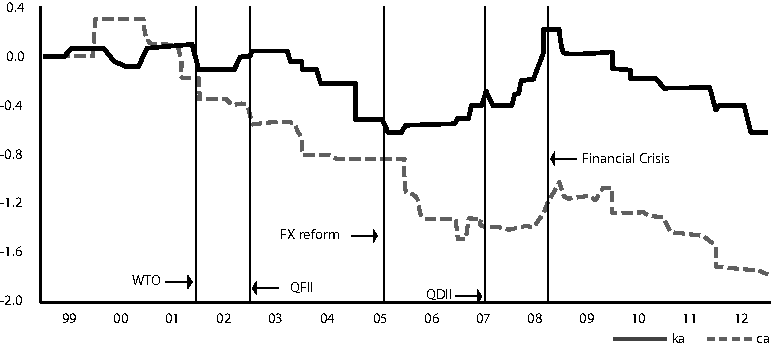
\includegraphics[scale=.9]{fig/capacc.pdf}
\caption{Index of Controls on China's Capital Account and Current Account}
\begin{figurenotes}
`ka' stands for capital account, and `ca' for current account. QFII refers to
Qualified Foreign Institutional Investor program launched in 2002, and QDII
refers to Qualified Domestic Institutional Investor program launched in 2007.
\end{figurenotes}
\begin{figurenotes}[Source]
\cite{chen2015}.
\end{figurenotes}
\label{fig:capacc}
\end{figure}

China started the Qualified Foreign Institutional Investor (QFII) program in 2002, 
which opened the channels for foreign institutional investors to access
China's domestic capital market, however the access quota was extremely limited.
In 2007, the counterpart of QFII -- the Qualified Domestic Institutional Investor (QDII)
program was launched for a selective domestic institutional investors to allow
them investing in foreign equity or bond markets. All cross-border portfolio
investment has been regulated under QFII and QDII programs until the establish
of Shanghai-Hong Kong Stock Connect in 2014, which opened another channel for
foreign investors to access domestic stock market via Hong Kong Stock Exchange.
The connect was furthered by Shenzhen-Hong Kong Stock Connect in late 2016. In
2016, China's central bank PBoC made a broad move to open the domestic
inter-bank bond market to foreign investors. Besides, China initiated to
experiment free capital account in Shanghai Free-Trade Zone in 2015. 

A cross-country comparison of capital account openness is illustrated by
the KAOPEN index proposed by \cite{chinn2008}. The index codifies the capital
account restrictions documented by IMF’s \textit{Annual Report on Exchange
Arrangements and Exchange Restrictions} (which monitors restrictions for
approximately 40 transactions under capital account). 
The indices measured in 2015 for a selected list of countries are shown 
in \autoref{fig:chinn-ito}. 
The index indicates that China's financial openness is much lower than 
developed countries and even some developing countries in Asia.
\autoref{fig:chinn-ito} also shows the gross asset plus liability to GDP ratio 
for each country as a \textit{de facto} measure of financial openness. 
The ratio indicates the financial openness in China may actually be better than 
what the KAOPEN index shows. But it is still far behind compared to high-income 
countries.

\begin{figure}[!htb]
\centering
\includegraphics[scale=1]{fig/chinn.pdf}
\caption{Chinn-Ito Index for Selected Countries}
\begin{figurenotes}
The primary axix is the Chinn-Ito financial openness index for 2015;
the secondary axis shows foreign asset plus liability to GDP ratio for 2013. 
The foreign asset plus liability to GDP ratio combines the scales of 
both assets and liabilities. The ratio of each individual country 
is therefore contributed by both inward and outward investment. 
\end{figurenotes}
\begin{figurenotes}[Source]
Chinn-Ito website, IMF, CICC Research. 
\end{figurenotes}
\label{fig:chinn-ito}
\end{figure}

Despite various liberalization reforms has been taken, China's capital account
is still under relatively heavy regulations compared with its current account.
There are quota management for almost all the available channels.
There is still a long way to go to achieve fully convertible 
capital account. \\


\subsection{Productive or prohibitive}

The controversy regarding financial liberalization and economic growth 
discussed in \Cref{sec:theory} extends to the financial policy issues 
in China as well. It would be improper to say the various financial regulations 
undertaken by the Chinese government have made no positive impact at all. 
For example,  the regulations on capital account protected 
the unfledged financial sector and prevented China from being adversely affected  
by the Asian Financial Crises as other South Asian countries.
But as the domestic financial institutions becoming mature, the negative effects 
of restrictive policies are predominating. 

\begin{figure}[!htb]
\centering
\includegraphics[scale=0.9]{fig/frep.pdf}
\caption{Financial Repressive Policies and Economic Growth}
\begin{figurenotes}
This figure shows the coefficients estimated by \cite{huang2011} of the effects  
of each repressive policy on economic growth. These repressive policies are 
state-owned banks in total bank loans (SOB), the share of the state sector in 
total outstanding loans (PCR), reserve requirement ratio (SRR), interest rate 
control (ICI), real deposit rate (RID) and capital account control (CAC).
FREP is the overall financial repression index that constructed from the above 
six variables. Among the result, the coefficients of SOB and CAC for 1979-99, 
SOB and RID for 2000-8 are statistically insignificant; other coefficients 
are significant for at least 5\% significance level.
\end{figurenotes}
\begin{figurenotes}[Source]
Based on estimations by \cite{huang2011}.
\end{figurenotes}
\label{fig:frep}
\end{figure}

This is illustrated by \cite{huang2011} who estimates the effects of various 
repressive financial policies undertaken in China -- 
deposit and interest rate control, capital account control,
reserve requirement ratio control and state-owned banks -- on economic growth 
(\autoref{fig:frep}).
Their findings suggest that the repressive policies exerted positive effects 
on economic growth in the early phase of development, but these positive effects 
mostly turned negative after 2000s. For example, they found interest rate controls  
initially prevented competition among banks and enhanced financial stability, 
but the negative effects such as reducing efficiency and hindering price 
discovery gradually dominated the benefits. Capital account restrictions that 
once protected the economy from international financial storms subsequently 
turned into the main obstacle for domestic investors accessing international 
capital markets to optimize their investment returns. 

China is now in a critical moment of its economic reform as the economy's growth  
is slowing after three decades of rapid expansion. It is also a critical 
time to rethink the past financial policies, as old policies may appear no longer 
suitable to tackle current problems. Though restrictive policies secured economic 
stability in the past, financial liberalization is becoming more relevant 
to improve efficiency and open new investment opportunities.
Efficient financial intuitions and markets will help ensure the 
quality of future investment, and facilitate the transformation 
from the current middle-income to a higher-income economy.\\


\section{Modelling Financial Reform}
\label{sec:model}

To project the potential impact of financial reform, we use 
a general equilibrium model to simulate the financial reform scenarios. 
The general equilibrium model used in this paper is based on the 
Global Trade Analysis Project (\citealp{gtap2016}), 
which is multi-region and multi-sector modelling project 
that has been widely used in global trade analysis. 
The latest version of GTAP database is Version 9a,
which contains micro- and macro-economic data for 
2004, 2007, 2011. 
In this paper, 2011 is taken as the reference year 
because it incorporates the economic adjustment after the GFC, 
although data for that year is influenced by the terms of trade 
boom in mining products such as iron ore and coal.

In terms of the general assumptions in GTAP, the model assumes regional 
households maximizing their Cobb-Douglas utility functions,  and regional 
firms minimizing their cost subject to constant returns to scale. 
Regional households are also assumed to have constant average propensity 
to save. In terms of global capital allocation, the model assumes 
that all savings are pooled into a ``global bank'' which ``allocates 
international capital flows in response to changes in regional rates 
of return'' \citep{gtap2016}. Besides, agricultural land, natural 
resources and labour endowment are assumed fixed in the model, while 
labour and capital are mobile across regional industries. 
The structure of the key elements of the GTAP model are briefly 
described in \autoref{fig:gtap-exp} and \autoref{fig:gtap-firm}.

\begin{figure}[!htb]
\centering
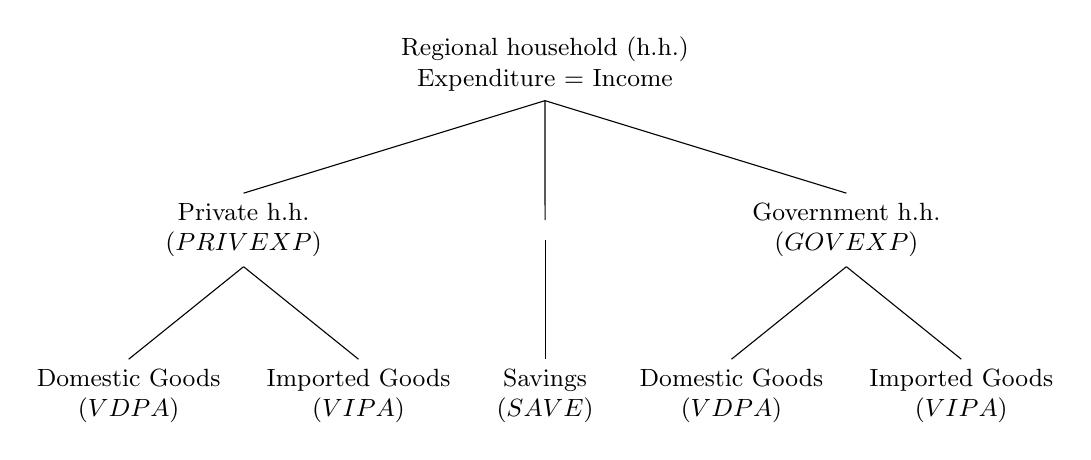
\begin{tikzpicture}[
   level distance=60pt,
   sibling distance=10pt,
   every tree node/.style={anchor=north},
   every node/.append style={align=center}  % <-- support line break
]
\tikzset{every tree node/.style={font=\small}}
\Tree 
    [.{Regional household (h.h.) \\ Expenditure = Income}
        [.{Private h.h. \\ ($PRIVEXP$)}
            [.{Domestic Goods \\ ($VDPA$)} ]
            [.{Imported Goods \\ ($VIPA$)} ]
        ]
        [.{}
            [.{Savings \\ ($SAVE$)} ]
        ]
        [.{Government h.h. \\ ($GOVEXP$)}
            [.{Domestic Goods \\ ($VDPA$)} ]
            [.{Imported Goods \\ ($VIPA$)} ]
        ]
    ]
\end{tikzpicture}
\caption{Regional Expenditure and Income}
\label{fig:gtap-exp}
\begin{minipage}{0.8\textwidth}
\notesize{\textit{Source}: The GTAP Modeling Framework, \cite{gtap2016}} 
\end{minipage}
\end{figure}

\begin{figure}[!htb]
\centering
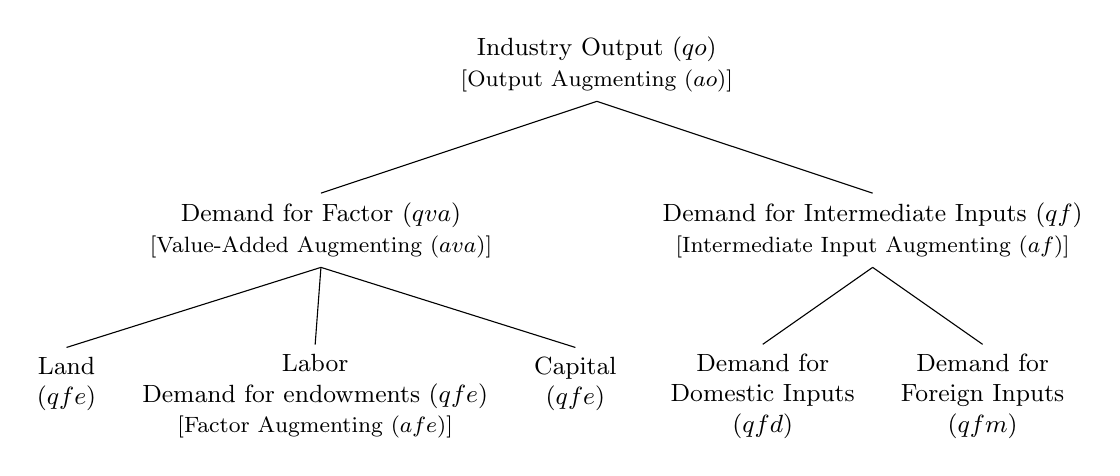
\begin{tikzpicture}[
   level distance=60pt,
   sibling distance=10pt,
   every tree node/.style={anchor=north},
   every node/.append style={align=center}  % <-- support line break
]
\tikzset{every tree node/.style={font=\small}}
\Tree 
    [.{Industry Output ($qo$) \\ 
       {\footnotesize [Output Augmenting ($ao$)]} }
        [.{Demand for Factor ($qva$) \\ 
           {\footnotesize [Value-Added Augmenting ($ava$)]} }
            [.{Land\\($qfe$)\\} ]
            [.{Labor\\Demand for endowments ($qfe$)\\
               {\footnotesize [Factor Augmenting ($afe$)]}} 
            ]
            [.{Capital\\($qfe$)\\} ]
        ]
        [.{Demand for Intermediate Inputs ($qf$) \\ 
           {\footnotesize [Intermediate Input Augmenting ($af$)]}}
            [.{Demand for \\Domestic Inputs \\($qfd$)} ]
            [.{Demand for \\Foreign Inputs \\($qfm$)} ]
        ]
    ]
\end{tikzpicture}
\caption{Firms Production Structure}
\label{fig:gtap-firm}
\begin{minipage}{0.8\textwidth}
\notesize{\textit{Source}: The GTAP Modeling Framework, \cite{gtap2016}} 
\end{minipage}
\end{figure}

The GTAP model used in this paper takes a comparative-static approach, 
where policy changes or productivity improvements are modelled as ``shocks''. 
The model takes a long-run perspective. 
Results are generated by comparing the economy before and after shocks, 
assuming full adjustment in the global economy.
Under the long-run assumption, capital stocks are assumed to adjust to 
maintain the required rate of return on capital fixed. 
The comparative-static model does not report any adjustment path 
after the shocks. 

For the purpose of this paper, all countries in the database are 
classified into five regions compring countries or country groups 
-- China (CHN), Australia (AUS), the United States (USA), 
European countries (EU), and the rest of the world (ROW). 
Industries are classified into 13 sectors.
The aggregation details can be found in \autoref{apx:agg}.

For the model being theoretical based, it is impossible to model every 
policy reform in real world directly. Instead several shocks to the 
model variables are simulated as proxies for the impacts of policy 
reforms. The shocks being simulated in this paper are:  
an increase in productivity of financial services, 
an increase in productivity of capital, and 
a reduction in required rate of return on capital.\\
%\newpage

\subsection{Simulation of an increase in productivity of finance service}
\label{sec:sim2}

As discussed in \Cref{sec:theory}, financial reforms that reduce restrictions 
on the financial system could improve the productivity of financial services. 
The productivity improvement of the financial sector is simulated by 
an incremental shock to the value-added augmenting technology and the 
intermediate input augmenting technology of financial service providers. 

% Suppose the financial sector has a production 
% function as \autoref{eqn:fin}, where $A_{Fin}$ is the coefficient 
% for value-added augmenting technology. The simulation assumes a 
% uniform 1 unit increase in $A_{Fin}$ for the financial sector.

% \begin{equation}
%     Y_{Fin} = A_{Fin} F(K,L,\dots)
%     \label{eqn:fin}
% \end{equation}

% The benefits that other industries receive from the productivity 
% increase of financial services are simulated through an increase 
% in the financial intermediate input augmenting technology. 
% Suppose Industry $i$ takes financial services as an intermediate 
% input in its production as in \autoref{eqn:firm}, where $\lambda_{Fin}$ 
% is the coefficient for financial intermediate input augmenting technology.
% The simulation applies a shock to coefficient $\lambda_{Fin}$ that increases 
% it by 1 unit uniformly. 

% \begin{equation}
%     Y_i = A_i F(\lambda_{Fin} Fin, L, \dots)
%     \label{eqn:firm}
% \end{equation}

% In GTAP, the simulation is done by shocking ``$ava(Fin)$" and ``$af(Fin)$" 
% if using the variable names as in \autoref{fig:gtap-firm}.

In the language of GTAP, the shock is done by 
\begin{alignat}{2}
    \label{eqn:p_fin}
    & \textrm{\textbf{Shock}}\ avaall (``Fin", ``\textrm{CHN}")\ 
        & = \textrm{\textbf{uniform}}\ 1.0 \footnotemark[1]\\
    & \textrm{\textbf{Shock}}\ afall (trad\_comm,``Fin", ``\textrm{CHN}")\ 
        & = \textrm{\textbf{uniform}}\ 1.0 \footnotemark[2]        
\end{alignat}%
\footnotetext[1]{ 
\noindent The variable $avaall(j,r)$ is the value-added augmenting 
technical change in sector $j$ of region $r$. 
While the variable $ava(j,r)$ illustrated in \autoref{fig:gtap-firm} stands for 
the average rate of value-added augmenting technical change in sector $j$ of region $r$.
The relationship between $avaall(j,r)$ and $ava(j,r)$ is given by:
$$ ava(j,r) = avasec(j) + avareg(r) + avaall(j,r) $$
where $avasec(j)$ is the value-added technical change of sector $j$ worldwide, 
$avareg(r)$ is the overall value-added technical change in region $r$.
The parameter ``$Fin$" represents the financial sector and ``CHN" is the country 
code for China. 
}
\footnotetext[2]{
\noindent The variable $afall(i,j,r)$ stands for intermediate input $i$ augmenting 
technical change by sector $j$ in region $r$.
The relationship between $afall(i,j,r)$ and $af(i,j,r)$ 
in \autoref{fig:gtap-firm} is defined in a similar way:
$$ af(i,j,r) = afcom(i) + afsec(j) + afreg(r) + afall(i,j,r) $$
where $afcom(i)$ and $afsec(j)$ are the worldwide intermediate technical change 
of input $i$ and of sector $j$ respectively, $afreg(r)$ is a regional 
shifter. $trad\_comm$ stands for all traded commodities.
}
\autoref{tab:sim-pfin} summarizes the simulation results for three key 
variables: real GDP, capital accumulation and trade balance to national income 
ratio. 
\begin{table}[!htb]
\begin{threeparttable}
\caption{Simulation Result of an Increase in 
Productivity of Finance Service in China}
\label{tab:sim-pfin}
\def\theadset{\def\arraytretch{1.5}}
\def\arraystretch{1.2}
\small
\begin{tabular}{lcccc}
\hline\hline
    & \thead{Read GDP\\\emph{\% change}} 
    & \thead{Capital accumulation\\\emph{\% change}} 
    & \thead{Trade balance to\\income ratio} \\
\hline
CHN & 4.392 &	11.130 & 0.018 \\
AUS & 0.132 &	0.256 & -0.003 \\
USA & 0.022 &	0.053 & -0.002 \\
EU  & 0.000 &	0.015 & -0.002 \\
ROW & 0.033 &	0.041 & -0.002 \\
\hline\hline
\end{tabular}
\begin{tablenotes}[para, flushleft]
\emph{Note:} Modelled as a uniform 1\% increase in value-added augmenting 
technology and a uniform 1\% increase in intermediate input augmenting 
technology in the financial sector.
The model is solved using Gragg's method; the accuracy requirement is set 
to that at least 99\% of the variables are accurate to at least 4 figures. 
The extrapolation accuracy shows that we can be confident for 6 figure 
accuracy for most variables.\\
\emph{Source:} Author estimated.
\end{tablenotes}
\end{threeparttable}
\end{table}

China is projected to increase its real GDP by 4.4\%, 
Australia by 0.13\%, USA by 0.02\%, 
while the impact of European countries as a whole is very small. 
Capital accumulation in China is projected to increase by 11.1\%.
Because a productivity improvement in financial services lowers the cost of 
financial resources of other industries, increasing industry competitiveness 
and demand for both labour and capital. 
Higher demand for capital raises investment above the level 
that would otherwise prevail. 
The model also projects an increase in trade balance to national income ratio 
for China, because improved competitiveness of the industries raises the volume 
of net exports. \\

\subsection{Simulation of an increase in productivity of capital}
\label{sec:sim3}

A well-functioning financial system allocates capital to the most productive 
and profitable firms.
Therefore, financial reforms that remove restrictions on financial system could,  
all else being equal, improve the productivity of capital in the Chinese economy. 

% Suppose the economy has a form of production function as in \autoref{eqn:proc}, 
% where $\lambda$ is the capital augmenting technology. 
% The following simulation applies a uniform 1 unit incremental shock to 
% $\lambda$ to project the overall increase in productivity of capital.

% \begin{equation}
%     Y = AF(\lambda K, L)
%     \label{eqn:proc}
% \end{equation}

% In the language of GTAP, the shock is applied to variable ``$afe(Capital)$".

The simulation is done by shocking capital augmenting technological change for 
all sectors in China by a uniform 1.0\% increment. 
\begin{equation}
    \label{eqn:p_cap}
    \textrm{\textbf{Shock}}\ afeall (``Capital", prod\_comm, ``\textrm{CHN}")\ 
     = \textrm{\textbf{uniform}}\ 1.0 \footnotemark[3]
\end{equation}
\footnotetext[3]{
The variable $afeall(i,j,r)$ is the factor $i$ augmenting technical change 
in sector $j$ in region $r$. 
The relationship between $afeall(i,j,r)$ and $afe(i,j,r)$ in \autoref{fig:gtap-firm}
is defined as:
$$ afe(i,j,r) = afecom(i) + afesec(j) + afereg(r) + afeall(i,j,r) $$
where $afecom(i)$ and $afesec(j)$ represent the worldwide technical change for 
input $i$ and sector $j$ respectively, $afereg(r)$ is a regional shifter. 
$prod\_comm$ stands for all traded commodities plus all capital goods. 
}
The simulation result is shown in \autoref{tab:sim-pcap}.
\begin{table}[!htb]
\begin{threeparttable}
\caption{Simulation Result of an Increase in 
Productivity of Capital in China}
\label{tab:sim-pcap}
\def\theadset{\def\arraytretch{1.5}}
\def\arraystretch{1.2}
\small
\begin{tabular}{lcccc}
\hline\hline
    & \thead{Read GDP\\\emph{\% change}} 
    & \thead{Capital accumulation\\\emph{\% change}} 
    & \thead{Trade balance to\\income ratio} \\
\hline
CHN & 4.807 &	11.624 & 0.018 \\
AUS & 0.142 &	0.279 & -0.003 \\
USA & 0.021 &	0.048 & -0.002 \\
EU  & -0.005 &	0.005 & -0.002 \\
ROW & 0.030 &	0.036 & -0.002 \\
\hline\hline
\end{tabular}
\begin{tablenotes}[para,flushleft]
\emph{Note:} Modelled as a uniform 1\% increase in capital augmenting 
technology for all sectors.
The model is solved using Gragg's method; the accuracy requirement is set 
to that at least 99\% of the variables are accurate to at least 4 figures. 
The extrapolation accuracy shows that we can be confident for 6 figure accuracy 
for most variables.\\
\emph{Source:} Author estimated.
\end{tablenotes}
\end{threeparttable}
\end{table}

The projected impacts of an overall 
improvement in the productivity of capital in China are similar to 
the result in \autoref{tab:sim-pfin} but the magnitude is even larger.
China's real GDP is projected to increase by 4.8\% and overall 
capital accumulation to increase by 11.6\%. Australia is also 
projected to have a larger increase in its real GDP (0.14\%) and 
capital accumulation (0.28\%). The impacts for all listed 
five countries and regions are overall positive except for Europe 
which is projected to have a slight decline in its real GDP 
(0.005\%) as its export competitiveness declines relative to 
that of China. \\

\subsection{Simulation of a reduction in required rate of return on capital}
\label{sec:sim1}

As discussed in \Cref{sec:theory} and \Cref{sec:facts}, various 
restrictions on financial system raise the overall cost of capital in the 
economy and the overall required rate of return on capital. Financial 
liberalization would potentially improve the efficiency of financial system 
in channelling funds to the most productive uses, lowering risk and reducing
the required return on capital relative to other economies.
This would induce more domestic investment from both local and oversea sourced 
funds, and boost economic growth in the long-run. 

% The classical mathematical model for return on capital and 
% capital accumulation is appended in Appendix 3.

% In GTAP, the required rate of return on capital in region $i$ ($rorc_i$)
% is modelled as the sum of a world average return rate ($rorc$) and a 
% regional risk premium ($r_i$).

% \begin{equation}
%     rorc_i = rorc + r_i
%     \label{eqn:rorc}
% \end{equation}

% The simulation applies a shock to $r_i$ -- reduce it   
% by 10\%. If taking the treasury yield as an illustration, 
% the recent rate for China is about 3.5\% and 2.2\% 
% for the US (as shown in \autoref{fig:t-yield}), a 10\% 
% reduction amounts to close the 30\% of the wedge. 

The simulation applies a 10\% reduction to the required rate of return 
on capital in China.
\begin{equation}
\label{eqn:rorc}
\textrm{\textbf{Shock}}\ f\_rorc(``\textrm{CHN}") = -10.0 \footnotemark[4]
\end{equation}
\footnotetext[4]{
In the GTAP model used in this paper, the modelling of the rate of return on capital 
is modified to incorporated regional risk premium. 
$$ rorc(r) = rorc\_r + f\_rorc(r) $$
where $rorc(r)$ stands for the percentage change of the required rate of 
return on capital in region $r$, 
$rorc\_r$ is the percentage change in the world average rate, 
and $f\_rorc(r)$ is the regional shifter (risk premium) for region $r$.
}
The simulation result is shown in \autoref{tab:sim-rorc}. 

\begin{table}[!htb]
\begin{threeparttable}
\caption{Simulation Result of a Reduction in Required Rate of 
Return on Capital in China}
\label{tab:sim-rorc}
\def\theadset{\def\arraytretch{1.5}}
\def\arraystretch{1.2}
\small
\begin{tabular}{lcccc}
\hline\hline
    & \thead{Read GDP\\\emph{\% change}} 
    & \thead{Capital accumulation\\\emph{\% change}} 
    & \thead{Trade balance to\\income ratio} \\
\hline
CHN & 4.088 &	10.824 & 0.018 \\
AUS & 0.127 &	0.245 & -0.003 \\
USA & 0.023 &	0.056 & -0.002 \\
EU  & 0.003 &	0.022 & -0.002 \\
ROW & 0.035 &	0.046 & -0.002 \\
\hline\hline
\end{tabular}
\begin{tablenotes}[para,flushleft]
\footnotesize
\emph{Note:} Modelled as a 10\% reduction in overall required rate of 
capital in China. 
The model is solved using Gragg's method; the accuracy requirement is set to that 
at least 99\% of the variables are accurate to at least 4 figures. 
The extrapolation accuracy shows that we can be confident for 6 figure accuracy 
for most variables.\\
\emph{Source:} Author estimated.
\end{tablenotes}
\end{threeparttable}
\end{table}

The real GDP are projected to increase for all five regions, with China 
as the largest beneficiary -- 4.1\% increase in real GDP, and 
Australia the second -- 0.13\% increase in real GDP.
The simulation also projects a 10.8\% increase in capital 
accumulation in China, in line with the classical theory. 
As to the trade balance, China is projected to have a larger trade surplus 
due to an increase in output induced by a reduction in required rate 
of return on capital. 

Compared with a similar simulation by \cite{gretton2015} using 2004 data, 
which projected a 5.7\% increase in real GDP for China, and a 0.06\% 
increase in real GDP for Australia, 
the result in \autoref{tab:sim-rorc} shows a smaller magnitude of projected increase 
in real GDP for China, but a doubled magnitude for Australia. 
The difference mainly arises from the difference in the reference years used in the 
simulations. 
During the years from 2004 to 2011, several financial reforms were undertaken in 
China (\Cref{sec:facts}) and the footprint of China in the global economy increased.
For terms of trade reasons, the potential impact of further liberalizing 
the financial system on the level of economic activity should be less
in 2011 than 2004.   
The larger magnitude of GDP growth of Australia is even more notable. 
One conjecture for the reason would be Australia's export to China 
increased dramatically during the years. 
An increasing in investment in China induced by the reduction of required 
rate of return on capital would therefore have a larger effect for Australia 
in 2011 than 2004. 

\subsection{Simulation of overall impact}
\label{sec:sim4}

In the reality, the impacts of financial reforms are unlike to be 
singular, but usually manifold -- a reduction in cost of capital,
an increase in productivity of financial sectors, or an increase 
in productivity of financial service or capital inputs, 
usually take place at the same time. 
A simulation that takes into account all the three 
potential impacts described in Section \ref{sec:sim2}-\ref{sec:sim1} 
is reported in \autoref{tab:sim-all}.

\begin{table}[!htb]
\begin{threeparttable}
\caption{Simulation Result of Overall Impact}
\label{tab:sim-all}
\def\theadset{\def\arraytretch{1.5}}
\def\arraystretch{1.2}
\small
\begin{tabular}{lcccc}
\hline\hline
    & \thead{Read GDP\\\emph{\% change}} 
    & \thead{Capital accumulation\\\emph{\% change}} 
    & \thead{Trade balance to\\income ratio} \\
\hline
CHN & 5.112 &	11.932 & 0.018 \\
AUS & 0.147 &	0.290  & -0.003 \\
USA & 0.020 &	0.045  & -0.002 \\
EU  & -0.008 &	-0.002 & -0.002 \\
ROW & 0.028 &	0.031  & -0.002 \\
\hline\hline
\end{tabular}
\begin{tablenotes}[para,flushleft]
\emph{Note:} 
% Modelled as a 10\% reduction in required rate of capital, 
% together with a uniform 1 point increase in value-added augmenting technology and  
% a uniform 1 point increase in intermediate input augmenting technology in  
% financial sector, and a uniform 1 point increase in capital augmenting technology 
% for all sectors.
Modelled by applying all shocks defined in \crefrange{eqn:p_fin}{eqn:rorc}.
The model is solved using Gragg's method; the accuracy requirement is set 
to that at least 99\% of the variables are accurate to at least 4 figures. 
The extrapolation accuracy shows that we can be confident for 6 figure accuracy 
for most variables.\\
\emph{Source:} Author estimated.
\end{tablenotes}
\end{threeparttable}
\end{table}

China is projected to 
increase its real GDP by 5.1\% and capital accumulation by 11.9
percent.
This total is not the simple aggregation of the individual shocks 
because the assumption that the policies do not change the supply of 
labour limits the expansion effect of improvements in the efficiency 
of financial markets and productivity in capital in production.
Australia is projected to increase its real GDP by 0.15\% 
and capital accumulation by 0.29\%. The impacts for the USA is less 
prominent, with a slightly 0.02 increase in real GDP and 0.05 in capital 
accumulation. European countries as a whole are projected to have a 
decline in both real GDP level and capital accumulation as the competitiveness 
of China increases relative to those economies. China is also 
projected to gain a trade surplus against other four countries or regions, 
because the productivity shocks would potentially improve the competitiveness 
of all its industries and thus increase net exports.  

An interesting finding is that the result projected by our GTAP general 
equilibrium model coincides with the result estimated by 
\citeauthor{huang2011}'s econometric model. 
According to \cite{huang2011},  the financial repression index (FREP) 
for China is estimated to 0.6 in 2008, and the semi-elasticity of 
GDP per capita to FREP is estimated to be 0.085.  
If China were to fully liberalize its financial system -- reducing the 
FREP to zero, the estimated GDP growth would be 5.1\%, 
which is of the same magnitude as projected in this paper. 

Further more, if China were to remove its restrictions interest rate, capital flows, 
and regulations favouring government designated projects, there would be 
redistributional effects of resources across different sectors in the 
economy. The sector imbalance described in \Cref{sec:facts} would 
be mitigated, and those repressed sectors would be expected to expand.
The projected sector performance is shown in \autoref{tab:sim-sector}.

\begin{table}[!htb]
\begin{threeparttable}
\caption{Simulation Result of Sector Output in China (\% Change)}
\label{tab:sim-sector}
\def\theadset{\def\arraytretch{2}}
\def\arraystretch{1.2}
\small
\begin{tabular}{lccccc}
\hline\hline
 & \thead{CHN} & \thead{AUS} & \thead{USA} & \thead{EU} & \thead{ROW} \\  
\hline
 Grains \& Crops 	            &2.702	&-0.011	&0.554	&0.238	&0.243 \\
 Livestock \& Fishing    	    &3.124	&0.716	&0.127	&0.205	&0.093 \\
 Mining      	                &4.188	&0.717	&0.328	&0.692	&0.502 \\
 Processed Food    	            &2.934	&-0.401	&0.018	&0.071	&0.050 \\
 Textiles    	                &5.619	&-2.558	&-0.976	&-1.175	&-1.413\\
 Light Manufacturing   	        &7.477	&-1.111	&-0.544	&-0.773	&-0.863\\
 Heavy Manufacturing   	        &7.477	&-1.903	&-0.493	&-0.359	&-0.813\\
 Construction       	        &2.734	&0.980	&0.783	&0.813	&0.760 \\
 Utilities       	            &5.841	&-0.277	&-0.062	&-0.117	&-0.185\\
 Transport \& Communication   	&5.467	&0.013	&0.040	&0.038	&0.053 \\
 Financial Services      	    &5.807	&0.182	&0.026	&0.066	&-0.003\\
 Dwellings         	            &6.307	&0.392	&0.075	&-0.006	&0.161 \\
 Other Services 	            &3.215	&0.192	&0.040	&0.022	&0.132 \\
\hline\hline
\end{tabular}
\begin{tablenotes}[para,flushleft]
\emph{Note:} 
% Modelled as a 10\% reduction in required rate of capital, 
% together with a uniform 1 point increase in value-added augmenting technology,  
% a uniform 1 point increase in financial intermediate input augmenting technology, 
% and a uniform 1 point increase in primary augmenting technology for capital.
Modelled by applying all shocks defined in \crefrange{eqn:p_fin}{eqn:rorc}.
The model is solved using Gragg's method; the accuracy requirement is set 
to that at least 99\% of the variables are accurate to at least 4 figures. 
The extrapolation accuracy shows that we can be confident for 6 figure accuracy 
for most variables.
\emph{Source:} Author estimated.
\end{tablenotes}
\end{threeparttable}
\end{table}

China is projected to have an increase in output levels for all sectors. 
It is worth noticing that the sectors that have been dominated by state-owned 
enterprises, such as manufacturing, utilities, transport, telecommunication and 
financial services are projected to increase more than others. This result is 
in line with the arguments posted in \Cref{sec:facts} that government 
designating resource allocation to state-owned enterprises reduces the 
efficiency and competitiveness of these sectors. 
Improved efficiency in these sectors is projected to lead to lower service 
prices and increases in demand for their outputs.
Other sectors also benefit as financial liberalization 
improves their accessibility to financial resources and reduces the overall 
cost of capital. Australia is projected to benefit overall and especially 
in its mining, livestock and fishing sectors. While the US is expected a gain 
in its construction, grains and crops sectors. The overall impact on Europe 
is projected to be negative, because its textile and manufacturing sectors 
would face more competition from Chinese imports and its exporters would 
face more competition in global markets.

It must be noted that these simulated results are projected to be the long-run 
equilibrium states. The adjustment path of each shock is not simulated in 
this model, and in reality, it depends on the specific reform agenda and 
the pace of the economy to adapt to the specific policy change. 
As pointed out in \Cref{sec:theory}, financial liberalization could 
exacerbate fluctuations or instability in an economy, which are not projected 
by this model. Further discussions on short-run instability issues will be 
considered in the following section.\\

\section{Policy Concerns}
\label{sec:policy}

In awareness of the importance of a liberalized financial system for better 
allocating resources to facilitate economic growth, the Chinese government 
has committed to further financial reforms in its 13th Five-Year Plan.
More specifically, the Chinese government pledged to
``improve financial institutions and market systems, promote the healthy
development of capital markets, improve monetary policy mechanisms, deepen reform
of the financial regulatory system, and refine our modern financial systems, thereby
improving the efficiency of the financial sector in serving the real economy 
as well as the financial sector ’s ability to support the transformation 
of China’s economy"\footnotemark[5].

\footnotetext[5]{13th Five-Year Plan for Economic and Social Development, Chapter 16.}

% ``to complete the establishment of financial institutions 
% and market mechanisms, to promote the healthy development of capital markets, 
% to establish monetary policy transmission mechanisms, to deepen reforms of 
% the financial regulation framework, to raise the efficiency of financial 
% services in serving the real sectors, and to effectively mitigate 
% financial risks''. \citep{joint-report2016}.

Undoubtedly, in recent years China has achieved remarkable progress 
liberalizing its financial system to freeing up bank deposits and 
lending interest rates (though the central bank still sets a reference rate), 
build up channels for cross-border portfolio investment through 
the Shanghai/Shenzhen-Hong Kong Stock Connects, open up the domestic 
bond market for foreign investors.
But more reforms have yet to resolve the country's financial 
repression syndrome. 
Though banks can float their interest rate freely, the 
monopoly of state-owned banks still stand in the way of a fully efficient 
allocation of financial resources, and the fragmentation of interest 
rates around institutional and regulatory constraints rather than 
commercial considerations in the economy remains. Even though restrictions 
on foreign portfolio investment were loosened, it did not 
meet the ever growing demands of domestic investors to diversify 
their portfolios. The stock market has yet to grow out of its cradle and 
still only plays a subsidiary role in financing new businesses. 
Though a registration-based initial offering system for the stock 
market has been on the agenda for many years, the reform is help up  
and currently IPOs still require regulatory approval.
Besides, the operating of pension funds is still in the nascent stages, 
and insurance industries are far from penetrating the economy 
to play a larger role in the management of risk from casualty events. 

While there are always tensions between financial liberalization 
and stability, in China the tension is even notable in its  
current financial situations. 
As economic growth is slowing, lower domestic investment 
returns and growing demand for foreign investment opportunities are 
raising concerns of capital flight if the capital account is freed up. 
As \cite{stiglitz2000} points out, pro-cyclical capital flows tend to 
exacerbate short-run fluctuations and destabilize the economy. 
Many developing countries have faced balance of payment crises 
when they liberalize their capital account 
(for example, the Asian crisis in 1997). 
For China, the exceptional volatility of the 2016 RMB exchange 
rate shows that the economy is still vulnerable during downturns. 
Although the central bank holds over \$3 trillion in 
foreign reserves, it would not counter massive capital transfers abroad 
(\$3 trillion foreign reserves only accounts for 15\%  of total national 
deposits).

% It would be difficult for the government to manage
% on the stability of the exchange rate if accompanied by the relative 
% stable current account and an plausible only modest increase 
% in capital inflows constrained by the underdeveloped domestic 
% financial markets. Nevertheless, it seems unlikely to cause a 
% full-blown financial crisis given he relative low level of 
% external debt and the large foreign exchange reserves. 

A more serious concern is raised on China's debt level --
the total debt to GDP ratio is estimated in 2016 to be almost 250\%, 
among which a large proportion is the lending to SOEs.
When the economy is slowing, rising nonperforming 
assets (NPA) could erode banks' balance sheet and threaten a 
banking system collapse. The situation is even more 
severe if considering the fast growing shadow banking sector.
The shadow banking services are provided by some financial 
intermediaries to circumvent the prudential regulations imposed 
on formal banks, adding more elements of risk into the financial system, 
with total assets estimated to approximately 65\% of China's GDP. 
In the context of the fragile banking system, a liberalization 
process must be undertaken deliberately but with caution to avoid 
the breakout of systematic risks in the banking system that transfer 
to the broader economy.

Yet, the short-run concerns of fluctuations should not 
impede the long-run effort to liberalize the financial system 
to realize the potential economic gains indicated by the 
projections above.
The question is how to gain the benefit of financial 
liberalization while limiting potential risks:
it will require the intelligence and artistry of Chinese 
policy markers. 
As \cite{mckibbin1999} suggested, 
instead of imposing restrictions and controls on the 
system, risk management is likely a better approach:  
``The alternative which is more likely to succeed is to allow 
reasonable mobility of financial capital but to improve the way 
in which domestic financial systems allocate capital within the 
economy. This includes improving systems of accountability, 
transparency in accounting systems, and monitoring the financial 
systems so a better evaluation of risk can be formulated".
\citeauthor{mckibbin1999}'s argument coincides with China's central
bank governor's notion of macro-prudential regulations on foreign 
debts and cross-border transactions \citep{zhou2012}. %\\


% \section{Conclusion}
% \label{sec:con}

% This paper stresses the importance of financial system to economic 
% growth and takes China as a specific examples. 
% Financial markets and intermediaries have been identified 
% to have the functions of mobilizing savings, allocating resources, 
% reducing transaction cost and information cost, facilitating liquidity, 
% ameliorating risk, exerting corporate controls, and therefore 
% facilitate economic growth. 

% China has been practising restrictive financial policies for many 
% years, including state-ownership of financial institutions, 
% interest-rate controls, industry entrance barriers, government 
% designating investments, and capital account restrictions. 
% However, these policies have caused inefficiency of resource 
% allocation and imbalance of sector development.

% The long-run impact of financial liberalization is simulated using 
% GTAP general equilibrium model. 
% The simulation assumes a reduction of required rate of return on 
% capital, an increase in productivity of financial services and 
% an increase in productivity of capital after financial reforms. 
% The simulation projects a remarkable increase in China's real GDP 
% by 5.1\% and an even larger increase in the total capital 
% accumulation by 11.9\%.
% Australia is projected to increase its real GDP by 0.15\%;  
% the United States is projected to increase its real GDP by 0.02 
%\%. While Europe is to slightly lose its real GDP by 0.008 
%\%, the rest of the world is to benefit by a 0.028\% 
% increase in average real GDP.
% The simulations also suggest productivity improvements for those 
% sectors dominated by state-own enterprises. 

% As to the policy side, considering the high level of debt and 
% asset bubble in housing market in China, financial liberalization 
% is not without risk. 
% Therefore, it is suggested that financial reforms be undertaken 
% together with prudential risk management.

\nocite{*}% include everything bibliography even though not been cited

\newpage
\bibliographystyle{aea}
\bibliography{ref}

% The appendix command is issued once, prior to all appendices, if any.
\appendix
\newpage
\section{Appendix: Aggregation Schemes}
\label{apx:agg}

\begin{table}[!htb]
\centering
\caption{Regional Classification}
\def\theadset{\def\arraytretch{1.5}}
\def\arraystretch{1.2}
\small
\begin{tabular}{ll}
\hline\hline
 Code & Countries \\
\hline
 CHN & China \\
 AUS & Australia \\
 USA & United States of America \\
 EU  & \makecell[l]{Austria Belgium Cyprus Czech Republic Denmark
                Estonia Finland France Germany Greece \\
                Ireland Italy Latvia Lithuania Luxembourg 
                Netherlands Poland Portugal Slovakia \\
                Spain Sweden Britain Bulgaria Croatia Romania
                Hungary Malta Slovenia }\\
 ROW & Other 108 countries in the world \\
\hline\hline
\end{tabular}
\end{table}

\begin{table}[!htb]
\centering
\caption{Industry Classification}
\def\theadset{\def\arraytretch{1.5}}
\def\arraystretch{1.2}
\small
\begin{tabular}{ll}
\hline\hline
 Sector Code & Industries \\
\hline
Grains \& Crops & \makecell[l]{Paddy rice, Wheat, Cereal grain, 
Vegetables, fruit, nuts, Oil seeds, \\ Sugar cane, sugar beet, 
Plant-based fibers, Crops, Forestry}
\\
Livestock \& Fishing & \makecell[l]{Cattle,sheep,goats,horses,
Animal products, Raw milk,Wool, \\ silk-worm cocoons,Fishing}
\\
Mining & \makecell[l]{Coal, Oil, Gas, Minerals}
\\
Processed food & \makecell[l]{Meat (cattle,sheep,goats,horse), 
Meat products,Dairy products,\\ Vegetable oils and fats,
Processed rice, Sugar, Food products, \\
Beverages and tobacco products}
\\
Textiles & \makecell[l]{Textiles, Wearing apparel}
\\
Light Manufacturing & \makecell[l]{Leather products, Wood products,
Paper products, publishing,\\ Manufactures}
\\
Heavy Manufacturing & \makecell[l]{Petroleum, coal products,
Chemical, rubber, plastic prods, \\Mineral products, 
Metals, Metal products, Motor vehicles and parts,\\Transport equipment, 
Electronic equipment, Ferrous metals,\\Machinery and equipment}
\\
Construction & Construction
\\
Utilities & \makecell[l]{Electricity, Gas manufacture, distribution,
Water}
\\
Transport \& Communication & \makecell[l]{Trade, Transport, Sea transport,
Air transport, Communication}
\\
Financial Services & \makecell[l]{Financial services, Insurance, 
Business services}
\\
Dwellings & Dwellings
\\ 
Other Services & \makecell[l]{Recreation and other services, 
PubAdmin/Defence/Health/Educat}
\\
\hline\hline
\end{tabular}
\end{table}

\newpage
\section{Appendix: CMF Code used in Simulations}
\begin{multicols}{2}
\begin{minted}[fontsize=\tiny]{text}
!   SHOCK_ALL.CMF
!   ================
!
!   Initial run for GTAP model:
!   *   define standard closure
!   *   perform price homogeneity test

auxiliary files = gtap_fin;

!  Solution method, accuracy
!  -------------------------
!  PC modelling set up
!  Using default method

Automatic accuracy = yes;
Accuracy percent = 99;
Subintervals = 4;    

check-on-read all = no; 
iz1 = yes;              ! Ignore zeros at step 1.
nds = yes;              ! Do no displays.
nrp = yes;              ! Don't reuse pivots.

!   base data
!   ---------

file gtapsets = GSETS.har;
file gtapparm = GPARAMS_std.har; 
file gtapdata = GBASEDATA.har ; !2011 DB, Latest from GTAP 

Identifier = gtap_fin.tab condensed using gtap_fin.sti ;

!   closure
!   -------

exogenous
    afall
    afcom
    afeall
    afecom
    afereg
    afesec
    afreg
    afsec
    ams
    aoall
    aoreg
    aosec
    atd
    atf
    atm
    ats
    au
    avaall
    avareg
    avasec
    cgdslack 
    endwslack
    incomeslack
    profitslack
  ! regional saving equals investment by E_SAVEPRICE
    psaveslack    
    tradslack
    pcgdswld
    dpgov
    dppriv
    dpsave
    pop
    qo(ENDW_COMM,REG)
    tm
    tms
    to
    tp
    tx
    txs  
;

Rest Endogenous ;

!  Exogenous variables for new equations
!  -------------------------------------

Exogenous
    rorc_r;      ! E_rorc2; global shift on ror;

!  Numeraire
!  ---------
!  en=ex change numeraire from pcgdswld to pfactwld

Swap pcgdswld = pfactwld; 

!  Closures
!  --------
!  Longer-run closure with national capital variable and rorc fixed. 

Swap qo("capital",reg) = f_rorc(reg) ;  !en=ex


!   Policy scenerios
!   ----------------

!  Scenario 1
!  ----------
!  Policy induced change in required rate of return on capital 

Shock f_rorc("CHN") =  -10.0;

!  Scenario 2
!  ----------
!  Technological change for the financial sector

! value added factor augmenting technological change to 
! the finance industry

Shock avaall("FinBus","CHN")  = uniform 1.0 ;   

! intermediate input augmenting technological change to 
! the finance industry

Shock afall(trad_comm,"FinBus","CHN") = uniform 1.0 ;       

!  Scenario 3
!  ----------
!  Capital augmenting technological change for all industries

Shock afeall("capital",prod_comm,"CHN") = uniform 1.0 ;  


!   verbal description
!   ------------------

model               = WASTE ;
version             = 0     ;
identifier          = TIME  ;
verbal description  = ON
                      THIS. ;

!   outputs
!   -------
equations file = standard;
extrapolation accuracy file = yes;
updated file gtapdata = <cmf>_data.har;

!
Solution         File = <cmf>.sl4 ;
Log              File = <cmf>.LOG ;

! Option is
CPU = YES ;
!

!   end of commands
!   ---------------
\end{minted}
\end{multicols}

\end{document}

% Word Count: 
% Total: 6233
% Excluding appendix: 5937